% !TeX spellcheck=en_GB
\section{Results}

This section contains our benchmarking results as well as a discussion of the results.

For each of the test categories, we measure performance for the three parallel versions, the outer parallel version executed sequentially on the CPU, and the sequential CPLEX java program. We have chosen instance sizes based on what could finish within at most a few minutes on our systems. The programs mentioned in Section \ref{priorwork} were typically tested on larger instances, but with a run-time of tens of minutes or even hours.

We plot the times in the same graphs for comparison. Note that comparison between the sequential and parallel versions might not be meaningful since they are executed on different machines and architectures. Additionally, different graphs should not be compared to each other as they use different scales.

\subsection{One big instance}
In this test category, we vary the size of the linear program while keeping the number of instances constant at one.

\begin{figure}[H]
	\centering
	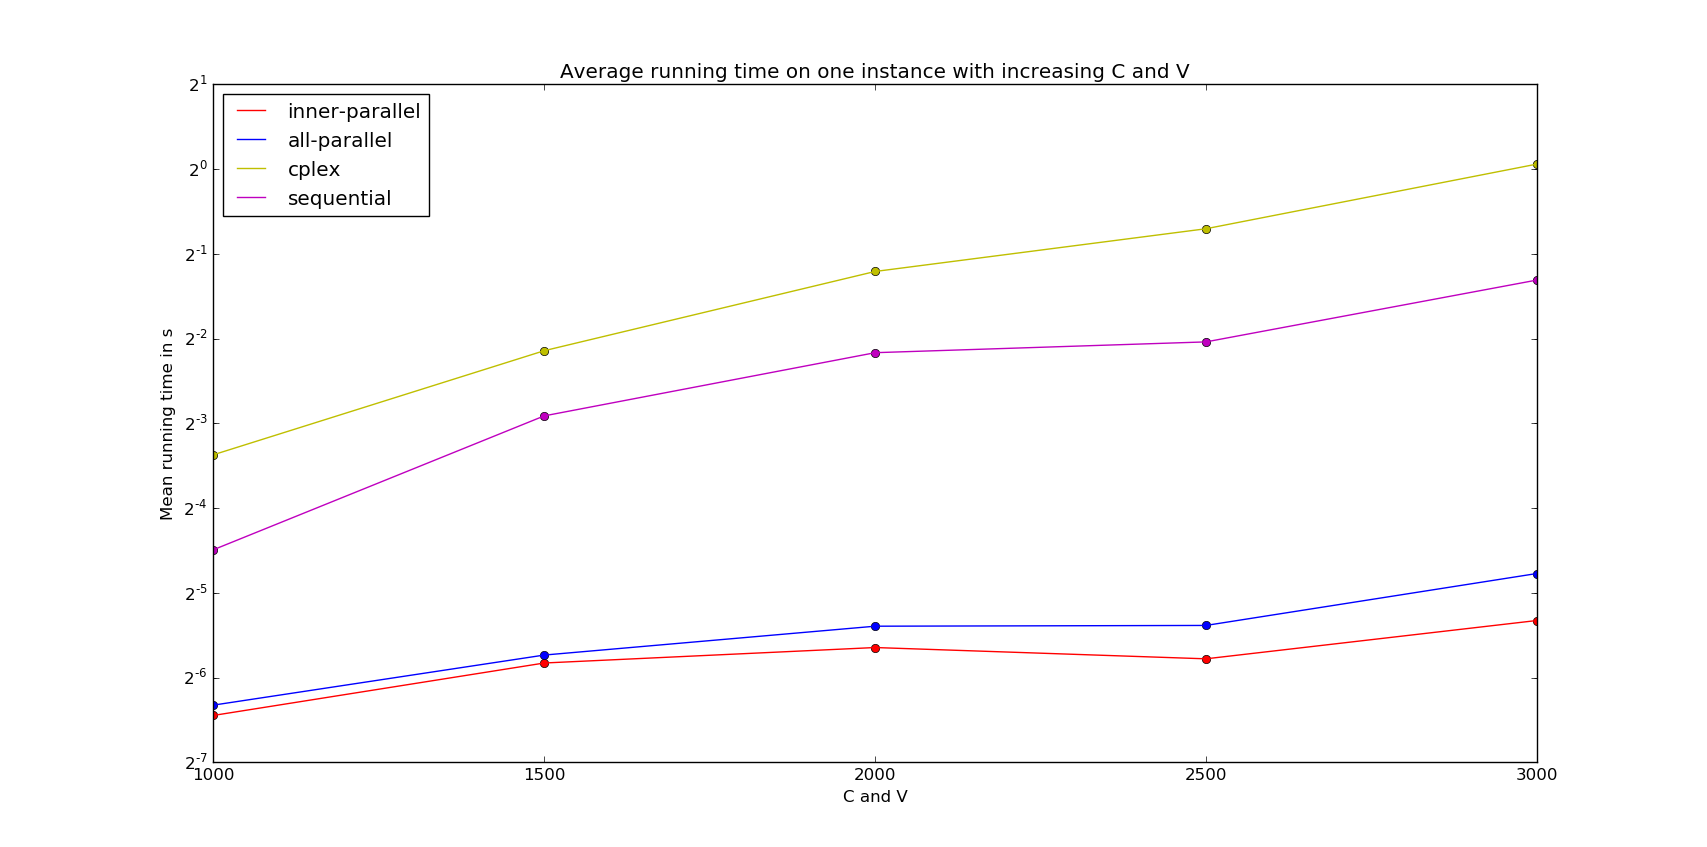
\includegraphics[width=\textwidth]{one-big}
	\caption{The average running time of the different implementations, with one instance with high number of C and V}
	\graphicspath{dir-list}
	\label{fig:one}
\end{figure}

\todo[inline]{Skal opdateres. Note to michael: change c and v to m and n. bigger text on graphs}

As seen in Figure \ref{fig:one}, the inner parallel version is the fastest implementation across all tests. This is expected since it is parallel on an instance while not having as much overhead as the fully parallel version. The outer parallel version executed on the GPU is not shown on the graph, because we were not able to run it on these tests. We encountered an OpenCL error, which might be due to memory allocation of big instances on a single GPU thread.
\todo{compare cpu with gpu (with reservations)}

\subsection{Many small instances}

In this test category, we vary the number of instances while keeping the sizes within a constant range of low values.

\begin{figure}[H]
	\centering
	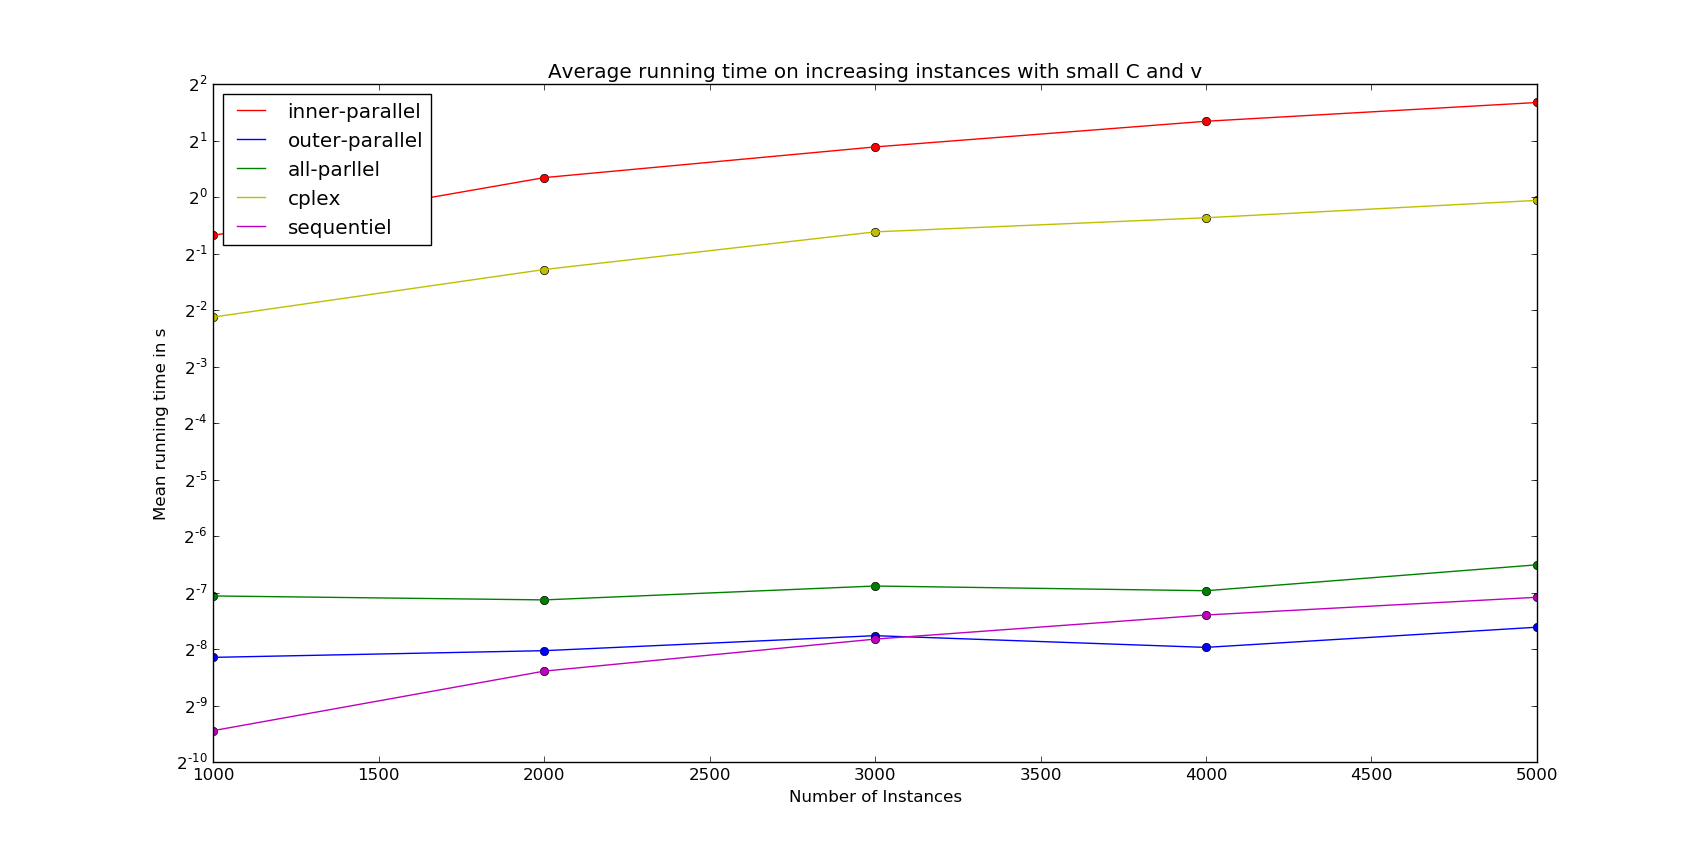
\includegraphics[width=\textwidth]{many-small}
	\caption{The average running time of the different implementations, on different sizes of N with a low number of C and V.}
	\graphicspath{dir-list}
	\label{fig-small}
\end{figure}
\todo[inline]{Skal opdaters}

As seen on Figure \ref{fig-small} the outer parallel version is the fastest for the largest number of instances. This is expected since it is parallel on the outer dimension, which is the dominant dimension in these test cases. The sequential version is the fastest for fewer than 3000 instances, but it has a more steep upwards slope, indicating that its growth would also exceed the fully parallel version.

Since each instance only requires relatively little work, the inner parallel version performs poorly. The fully parallel version performs well, which is expected since it is also parallel in the outer dimension, but it is clear that the overhead for flattening the nested parallelism makes it slower than the only outer parallel version.

CPLEX performs badly here which is possibly due to the pure overhead in solving a single instance. We also note that the assumptions in our implementations are not present in CPLEX which may also be why there is extra overhead in CPLEX.

\subsection{Many big instances}
In this test category, we vary the number of instances while keeping the sizes within a constant range of high values.

\begin{figure}[H]
	\centering
	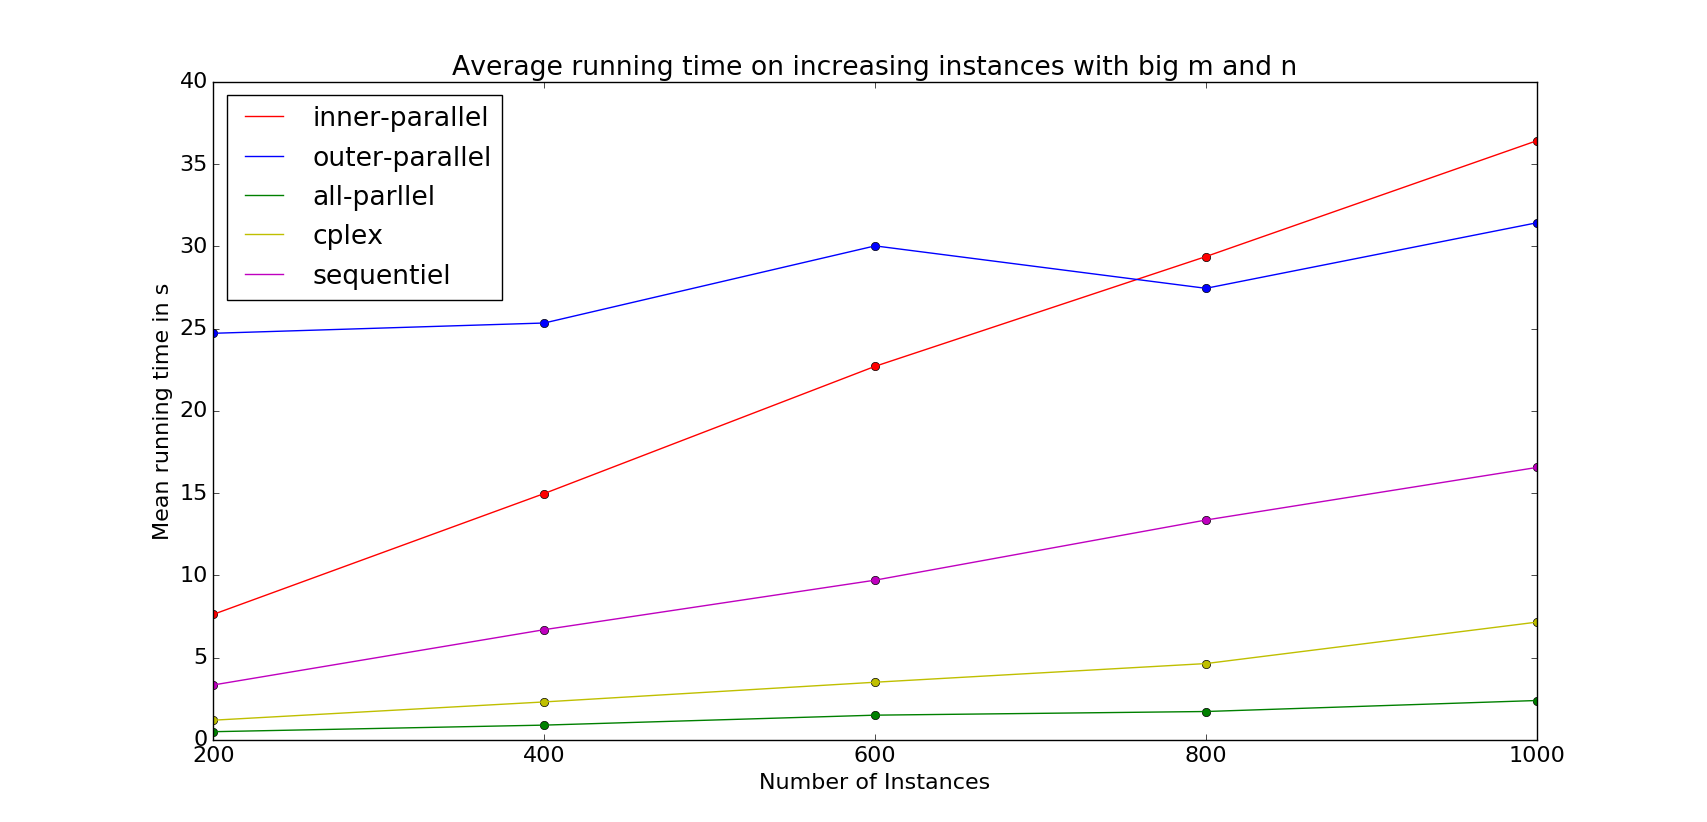
\includegraphics[width=\textwidth]{many-big}
	\caption{The average running time of the different implementations, on different sizes of N with high numbers of C and V}
	\graphicspath{dir-list}
	\label{fig-big}
\end{figure}
\todo[inline]{Skal opdaters}

As seen in Figure \ref{fig-big} the fully parallel implementation is the fastest. This was expected since it is the implementation with the highest level of parallelism on both dimensions. Since both dimensions are large, it effectively utilises the number of threads to its fullest and the overhead becomes negligible. The inner parallel version does comparatively well since the sizes of the instances allow it to utilise the GPU significantly. The outer parallel version seems to be limited by the time needed to solve each instance.

\subsection{Many instances of varying size}
In this test category, we vary the number of instances while keeping the sizes within a constant, but broad range of values.

\begin{figure}[H]
	\centering
	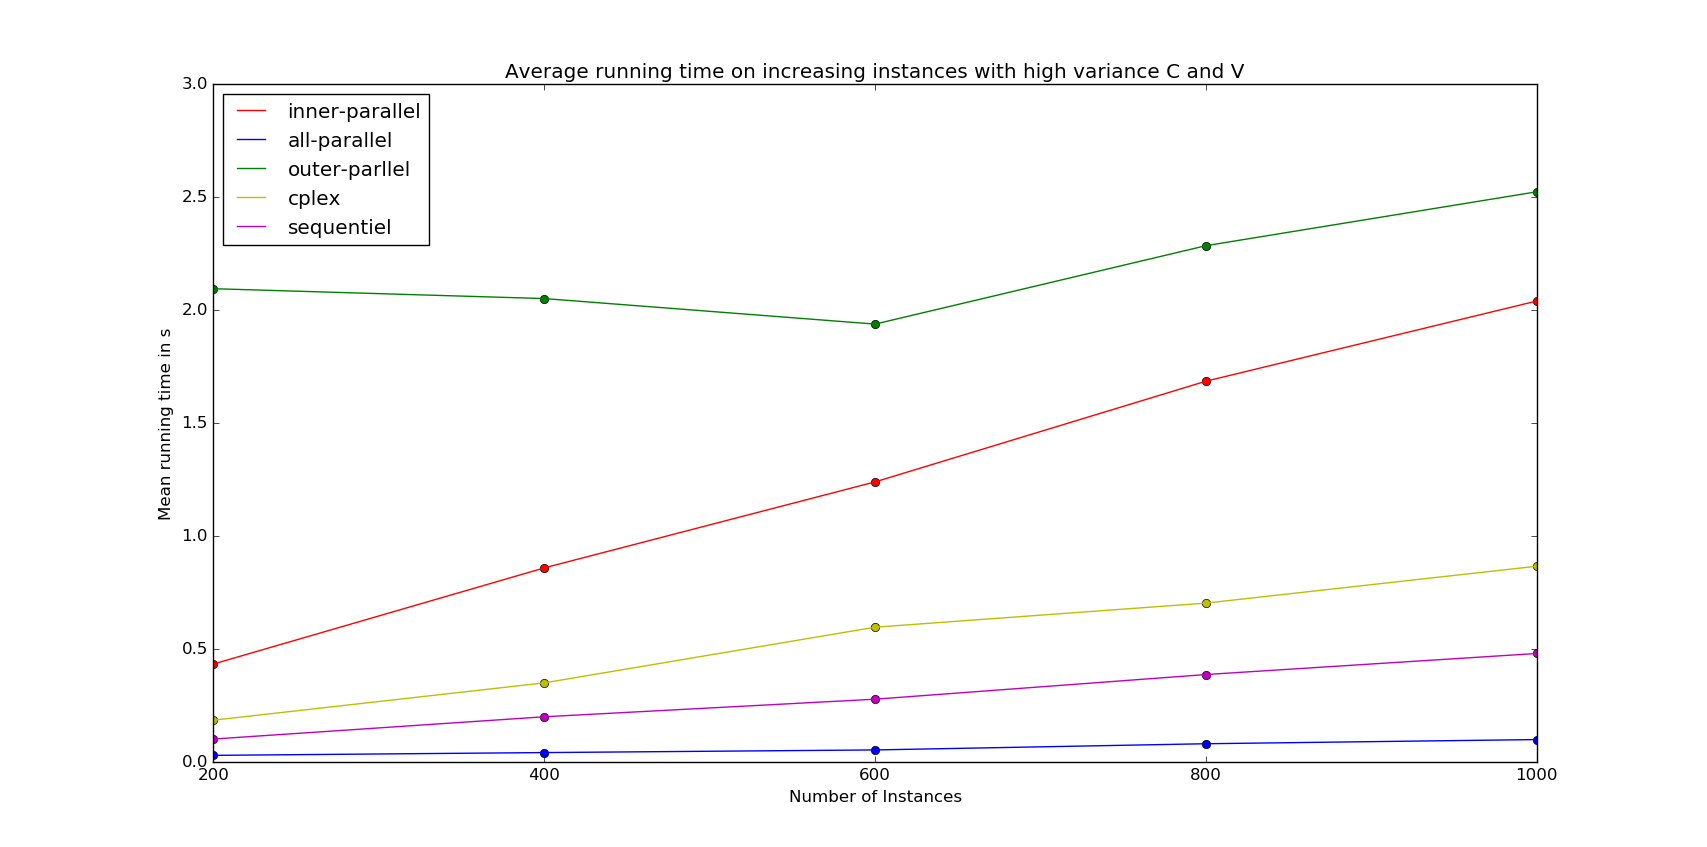
\includegraphics[width=\textwidth]{many-varying}
	\caption{The average running time of the different implementations, on different sizes of N with C and V varying a lot.}
	\graphicspath{dir-list}
	\label{fig-vary}
\end{figure}

\todo{parameters in caption}
\todo[inline]{Skal opdaters}
As seen in Figure \ref{fig-vary} the fully parallel version shows its strength. As in the category with many big instances, it is capable of maintaining high GPU utilisation without getting bottlenecked. The inner parallel version also has similar performance to the case with many big instances. This could be because all the arrays are padded and therefore will have size as big as the biggest possible instance. The outer parallel version performs better than in the case with many big instances.